% chktex-file 8
%   Allow dashes
% chktex-file 17
%   Don't require matching number of brackets and parentheses
% chktex-file 11
%   Allow ellipsis
% chktex-file 44
%   Allow regex
\documentclass{article}
\usepackage{amsmath}
\usepackage{graphicx}
\usepackage[a4paper, margin=1in]{geometry}

\title{Paleoclimate Causal Inference DAG Formulation}
\author{Jasmin Billingsley \\ Viktor Butkovich \\ Kristin Nyenhuis}
\date{October 29, 2025}
\begin{document}

\maketitle

\section*{DAG Variables}
\begin{itemize}
    \item Let Y be anomaly (outcome), the deviation of global temperature from the 1961-1990 Berkeley Earth baseline.
    \item Let A designate CO2 concentration.
    \item Let X1 designate a variable representing the combined effect of the Milankovitch orbital parameters:
    \begin{enumerate}
        \item Eccentricity
        \item Obliquity
        \item Perihelion
        \item $65^\circ\mathrm{N}$ Insolation
        \item Global Insolation
    \end{enumerate}
    \item Let X2 designate the Beryllium-10 concentration, a proxy for cosmic ray flux.
    \item Let X3 designate VADM, a proxy for geomagnetic field strength.
    \item Let X4 designate solar modulation, a derived value based on Be-10 concentration and VADM, representing the effect of solar activity on cosmic ray flux.
    \item Let X5 designate CO2 radiative forcing (treatment), a derived value based on CO2 concentration to represent the effect of CO2 on global temperature.
    \item Let U1 designate the true global anomaly, for which anomaly is a proxy measurement from oxygen isotope ratios, pollen counts, etc.
    \item Let U2 designate magnetic field strength, for which VADM is a proxy measurement from sediment cores.
    \item Let U3 designate cosmic ray flux.
\end{itemize}

\section*{DAG Links}
\begin{itemize}
    \item $A \to X5$: CO2 radiative forcing is directly derived from CO2 concentration.
    \item $X1 \to U1$: Milankovitch cycles are exogeneous variables that directly affect global temperatures through season length and sunlight received.
    \item $X1 \to A$: Milankovitch cycles affect CO2 concentrations through positive feedback mechanisms during glaciation and deglaciation.
    \item $X4 \to U3$: Solar modulation affects cosmic ray flux.
    \item $X5 \to U1$: CO2 radiative forcing directly affects global temperatures.
    \item $U1 \to Y$: True global anomaly affects measured anomaly proxies.
    \item $U2 \to X3$: Magnetic field strength affects VADM measurements.
    \item $U2 \to U3$: Magnetic field strength affects cosmic ray flux.
    \item $U3 \to X2$: Cosmic ray flux affects Be-10 concentration measurements.
    \item $U3 \to U1$: Cosmic ray flux affects global temperatures through cloud formation.
    \item $U3 \to A$: Cosmic ray flux affects CO2 concentrations through positive feedback mechanisms during glaciation and deglaciation.
\end{itemize}

\begin{figure}[!ht]
    \centering
    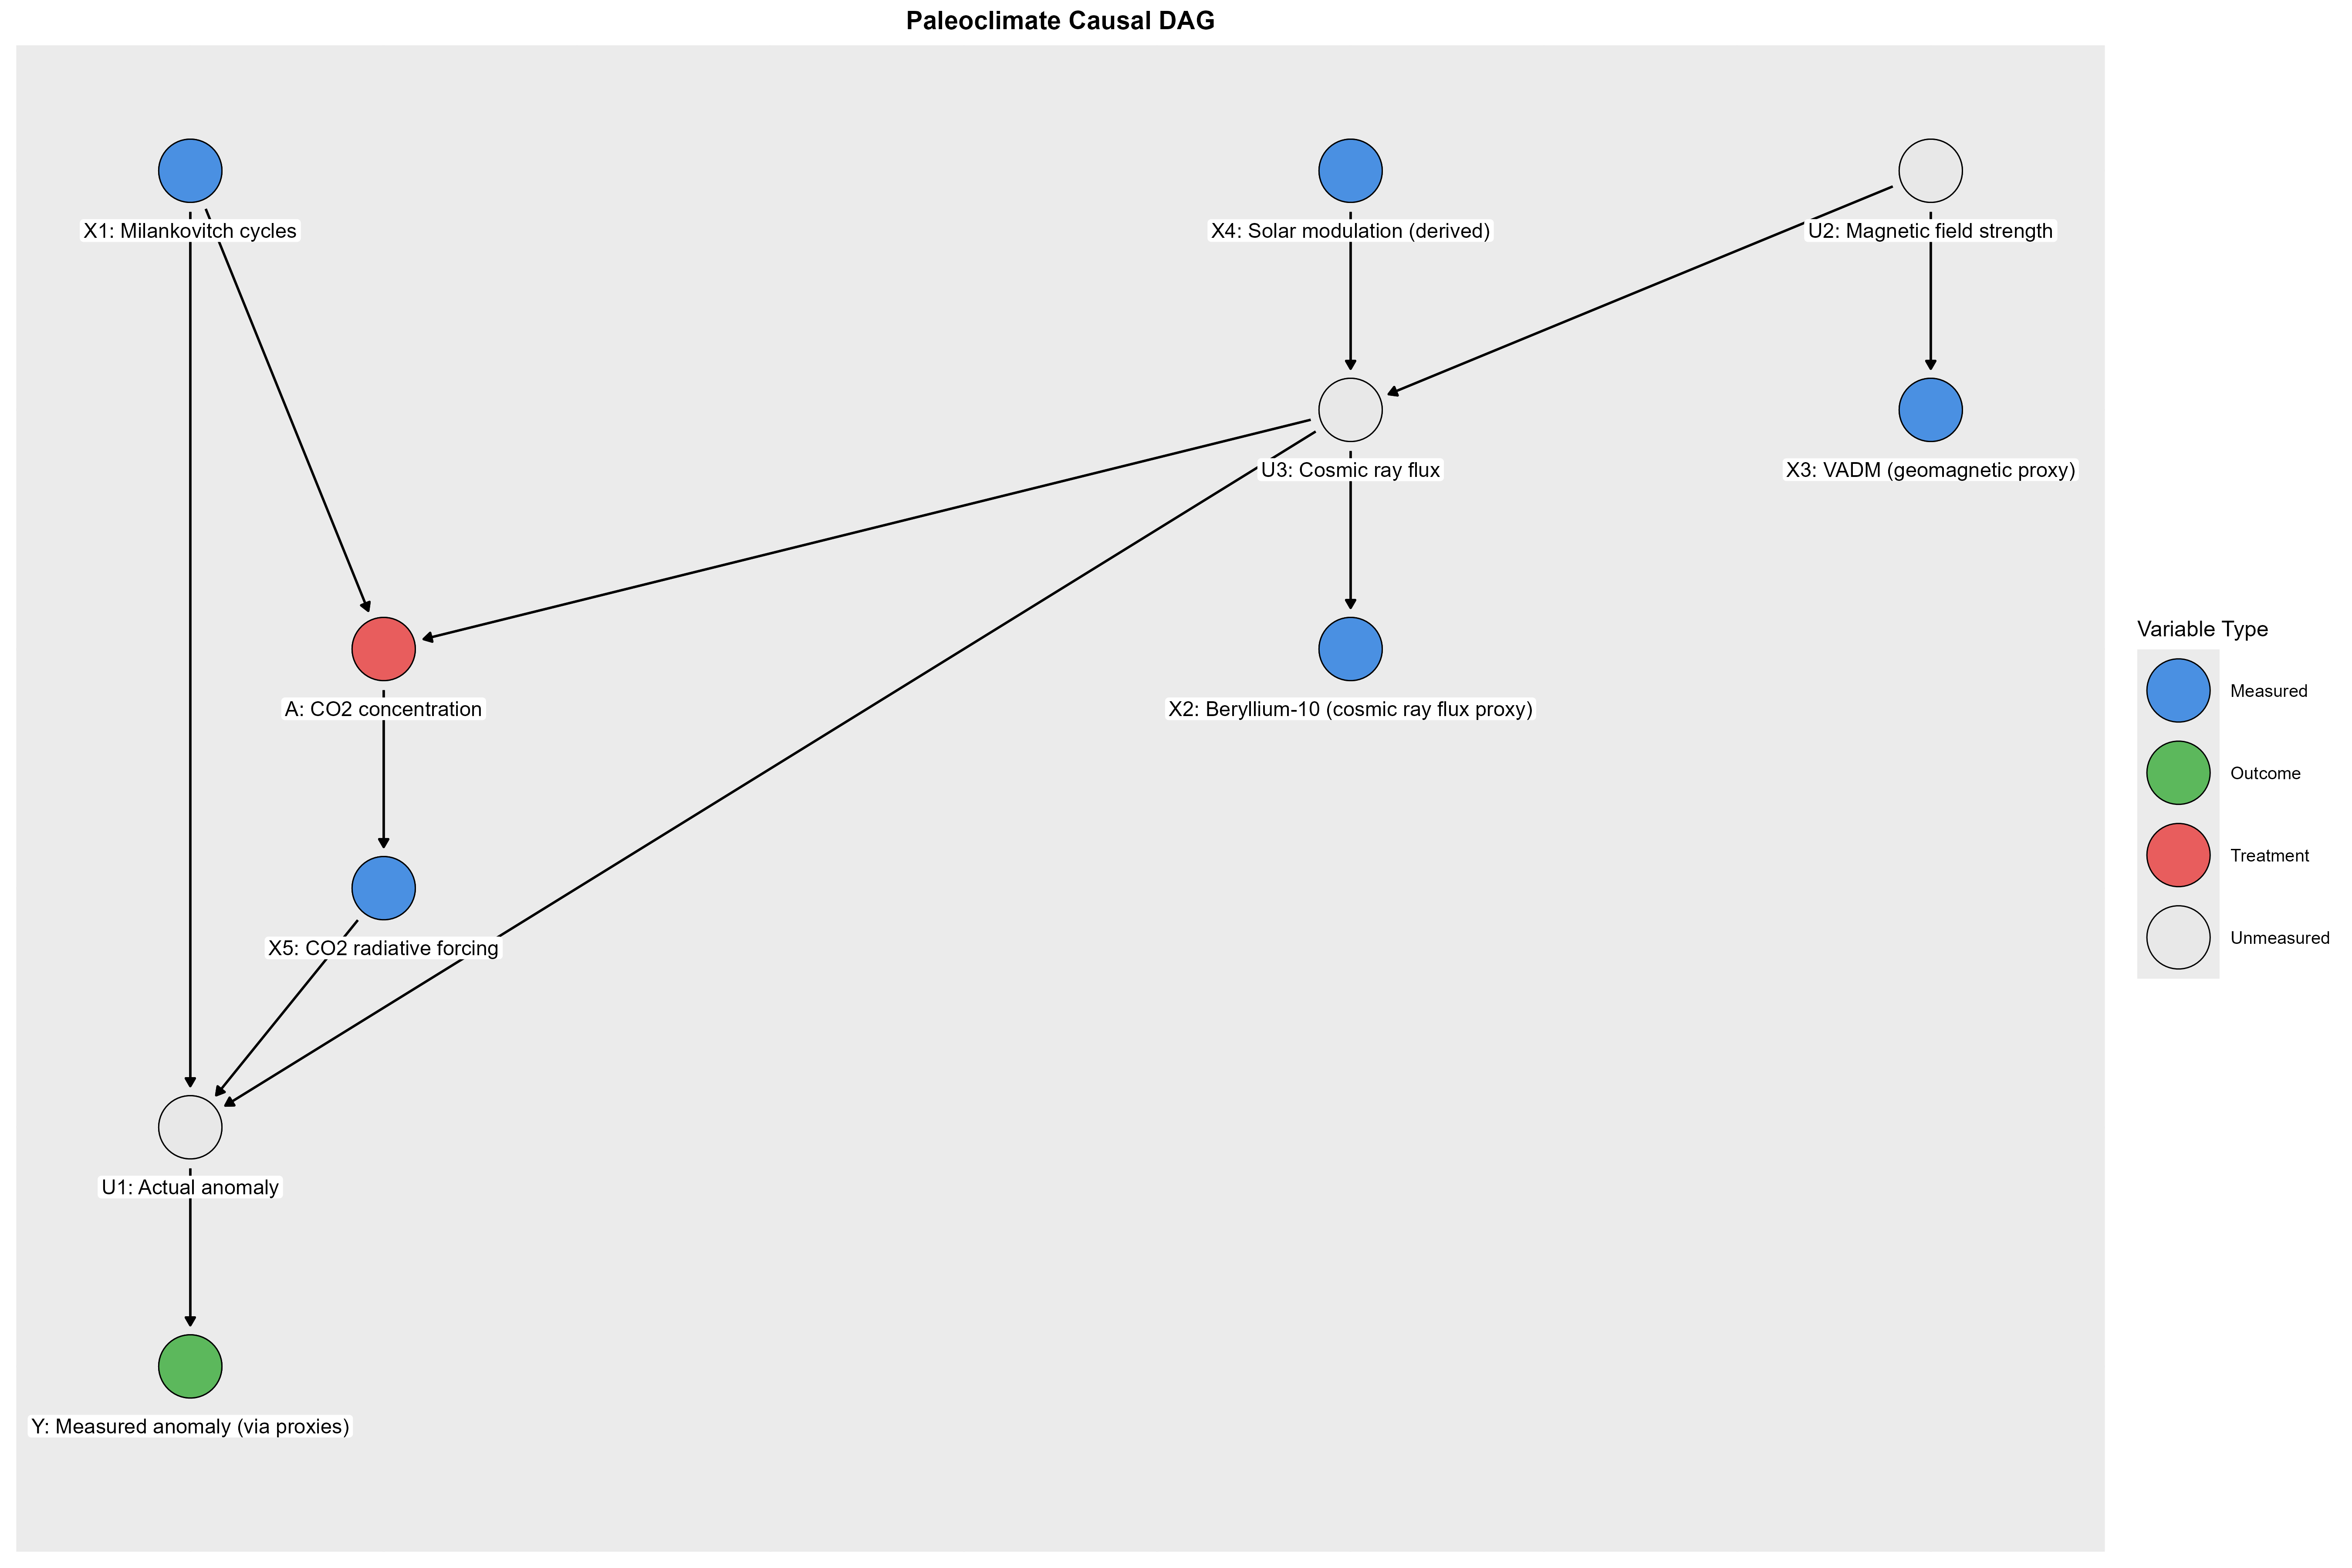
\includegraphics[width=500px]{../Outputs/Paleoclimate_Causal_DAG.png}
    \caption{DAG Graphical Representation}
\end{figure}

\end{document}